\begin{figure}[h]
	%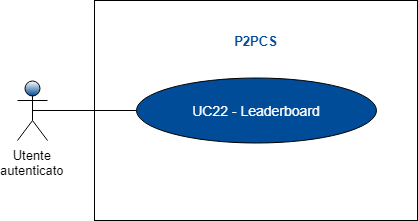
\includegraphics[width=11cm]{res/images/UC22Leaderboard.png}
	\centering
	\caption{Schema generale: leaderboard}
\end{figure}
\subsubsection{UC22 - Leaderboard}
\begin{itemize}
	\item \textbf{Attori Primari}: utente autenticato;
	\item \textbf{Descrizione}: dall'interno della sua area personale, l'utente può visualizzare la classifica dei migliori utenti;
	\item \textbf{Scenario principale}: l'utente apre la sezione \textit{Gestione Profilo} [UC14] e consulta la classifica utenti;
	\item \textbf{Precondizione}: l'applicazione rende disponibile la visualizzazione della Leaderboard\glosp;
	\item \textbf{Postcondizione}: l'utente autenticato ha visualizzato la leaderboard.
\end{itemize}

